\documentclass[12pt,twoside,notitlepage]{report}
\usepackage{a4wide}
\usepackage{graphicx}
\usepackage{listings}
\usepackage{color}
\usepackage{mathtools}
\usepackage{algorithm}
\usepackage{algpseudocode}
\usepackage{url}
\usepackage{pgfplots}
\allowdisplaybreaks
\renewcommand{\algorithmicforall}{\textbf{for each}}

\raggedbottom                           % try to avoid widows and orphans
\sloppy
\clubpenalty1000%
\widowpenalty1000%

\addtolength{\oddsidemargin}{6mm}       % adjust margins
\addtolength{\evensidemargin}{-8mm}

\renewcommand{\baselinestretch}{1.1}    % adjust line spacing to make
                                        % more readable

\DeclareMathOperator*{\argmin}{argmin}

\definecolor{dkgreen}{rgb}{0,0.6,0}
\definecolor{gray}{rgb}{0.5,0.5,0.5}
\definecolor{mauve}{rgb}{0.58,0,0.82}

\lstset{frame=tb,
  language=C,
  aboveskip=3mm,
  belowskip=3mm,
  showstringspaces=false,
  columns=flexible,
  basicstyle={\small\ttfamily},
  numbers=none,
  numberstyle=\tiny\color{gray},
  keywordstyle=\color{blue},
  commentstyle=\color{dkgreen},
  stringstyle=\color{mauve},
  breaklines=true,
  breakatwhitespace=true
  tabsize=3
}

\parindent 0pt
\parskip 6pt

\begin{document}


\pagestyle{empty}

\hfill{\LARGE \bf Vit Huang}

\vspace*{60mm}
\begin{center}
\Huge
{\bf Real-time Non-Photorealistic Rendering in the Style of Pixel Art} \\
\vspace*{5mm}
Computer Science Tripos Part II \\
\vspace*{5mm}
Churchill College \\
\vspace*{5mm}
\today  % today's date
\end{center}

\cleardoublepage

\setcounter{page}{1}
\pagestyle{plain}

\chapter*{Proforma}

{\large
\begin{tabular}{ll}
Name:               & \bf Vit Huang                       \\
College:            & \bf Churchill College                     \\
Project Title:      & \bf Real-time Non-Photorealistic Rendering \\
					& \bf in the Style of Pixel Art \\
Examination:        & \bf Computer Science Tripos Part II        \\
Word Count:         & \bf 10690 \\
Project Originator: & Vit Huang                    \\
Supervisor:         & Dr A.~Benton                   \\ 
\end{tabular}
}

\section*{Original Aims of the Project}

To design and implement a system to render 3D models in a way that emulates the non-photorealistic style of pixel art, including common features unique to the art form. The system should be capable of rendering a complex scene in real time as the scene animates.

\section*{Work Completed}

A system that renders a textured 3D model file in a style emulating pixel art, in the form of a web page using WebGL for graphics hardware acceleration. The system is capable of rendering a scene, containing tens of thousands of polygons and at a resolution of 1024$\times$1024 pixels, 60 times a second.

\section*{Special Difficulties}

None.
 
\newpage
\section*{Declaration}

I, Vit Huang of Churchill College, being a candidate for Part II of the Computer Science Tripos, hereby declare that this dissertation and the work described in it are my own work, unaided except as may be specified below, and that the dissertation does not contain material that has already been used to any substantial extent for a comparable purpose.

\bigskip
\leftline{Signed}

\medskip
\leftline{Date}

\cleardoublepage

\tableofcontents

\chapter{Introduction}

\section{Pixel Art}

As computer graphics technology has evolved over the years, so have the art styles used in applications such as user interfaces and computer and video games. Early technology only allowed for the use of simple black-and-white \textit{bitmaps} or \textit{vector graphics}, all performed on the main processor. Bitmaps (also known as \textit{raster images}) consist of a 2D array, where each array element maps to one screen pixel; vector graphics are described by a mathematical function, and rendered either using a specialised device such as an oscilloscope, or by converting the vector image into a bitmap (a process called \textit{rasterisation}).

The limitations of display technology combined with the cost of rendering meant that artistic concepts had to be communicated using very few colours in very few pixels, leading to a distinctive blocky style -- the first form of \textit{pixel art}.

In order to combine the advantages of 3D computer graphics with the aesthetic style of 2D pixel art, I have made use of modern graphics technology to produce a GLSL shader program that renders a 3D model using techniques and limitations commonly used in pixel art. In order to reap full benefits from 3D techniques, the program runs in real-time, capable of rendering a complex scene with a movable camera at a smooth frame rate. This is impossible to achieve with hand-drawn pixel art, and allows developers wishing to use the pixel art style more flexibility than was previously possible.

\begin{figure}[h!]
\centering
\includegraphics{spaceinvadersprite}
\caption{An example of early pixel art, from \textit{Space Invaders} (1978) by Tomohiro Nishikado}
\label{fig:spaceinvader}
\end{figure}

The first usage of pixel art was for black-and-white bitmap icons in early graphical user interfaces, starting with Engelbart's `Mother of All Demos' in 1968~\cite{Engelbart:1968:RCA:1476589.1476645}. This type of pixel art usually depicted mundane items that might be present on a physical desktop, such as stacks of papers. However, this changed with the rise of video games, such as Space Invaders (pictured in Figure~\ref{fig:spaceinvader}). Very early games did not feature pixel art -- games such as \textit{Tennis for Two} (1958; William Higinbotham) and \textit{Spacewar} (1961; Steve Russell) were played on oscilloscope screens, with graphics traced out by modifying the electron beam's path. However, as the industry grew, developers started to improve the graphics presented to the user in order to gain an edge over their competitors. Consumer video game hardware hooked into pixel-based televisions rather than oscilloscopes, so pixel art similar to that in Figure~\ref{fig:spaceinvader} quickly fell into widespread use. As technology and processing power steadily progressed, artists were free to create more and more detailed art.

The use of pixel art in games peaked in the mid-1990s, with games consoles such as Nintendo's SNES (Super Nintendo Entertainment System) using hardware optimised to display many detailed pixel art \textit{sprites} simultaneously. However, pixel art was still defined by the same limitations that spawned it. Despite the vastly more powerful hardware, there were still limitations on the size of both the sprite itself and the \textit{palette} its colours were drawn from; a sprite is a 2D image that forms part of a scene, such as an object or character, while a palette is a vector of colours that are used in a sprite. Sprites were stored as a 2D array of integers, where each element was an index into the sprite's palette. The size of the array allocated per sprite put a limit on the size, and the size per integer index limited the number of colours that could be in the palette. For example, the SNES had an output resolution of 256x224 pixels, with the most commonly-used operating mode of the graphics chip using 4 bits per pixel and thus supporting 16 colours per sprite (including the transparent background colour).

\begin{figure}[h!]
\centering
\includegraphics{linksprite}
\caption{The evolution of pixel art: several sprites depicting the character `Link' from \textit{The Legend of Zelda} series (Nintendo, 1986-2005)}
\label{fig:link}
\end{figure}

Due to these limitations, pixel art is identified by several features common across all eras. Each image has a relatively small size (the pixel art figures presented are enlarged using nearest neighbour magnification for clarity) and draws the colour of each pixel exclusively from a fixed palette. This leads to quirks usually not seen in other art styles, such as visible `banding' as a result of quantising a smooth gradient to a small palette (as seen on Link's hair in the rightmost sprite in Figure~\ref{fig:link}), or the use of a single shade of colour for parts of the subject that might actually be different colours in the original concept (compare the colours of Link's hair, shield, and shoes in the leftmost sprite).

In addition, parts of the subject are often outlined with a one-pixel-wide border in order to make them stand out from the background and from each other (notice how much easier it is to resolve the features of the second and third examples of Link, which use this technique, than the first, which does not). Originally this was done with a single colour (usually black, as seen in the middle sprite in Figure~\ref{fig:link}), but as the style evolved, artists started to replace this with darker shades of the base colour of the object, resulting in a softer look that preserved the purpose of the technique (compare the edge of Link's hair in the middle and rightmost sprites).

Finally, smaller features on the subject are often enlarged in order to make them identifiable in the small number of pixels available; in the rightmost example, Link's shoes have been enlarged relative to their physical proportions in order to make his walking animation clearer, and the hair at the sides of his head has been widened to allow for it to be outlined to separate it from his face and the background.

\begin{figure}[h!]
\centering
\includegraphics{dithering}
\caption{Examples of types of dithering (from Wikimedia Commons)}
\end{figure}

In order to produce the illusion of colours in addition to those already in the palette, a technique named \textit{dithering} was used. The image would contain a pattern of pixels of different colours. The cathode ray tube displays at the time used a shadow mask in order to ensure the three electron beams could only strike and illuminate one colour of subpixel each. However, the beams themselves diverged slightly, so each would slightly illuminate surrounding subpixels of the same colour. This resulted in neighbouring pixels blurring together, causing dithered areas to appear closer to the uniform colour formed by blending the dithered colours. Although modern displays no longer produce this effect, the high resolutions in use now pack the pixels closely enough that it is difficult for the human eye to distinguish separate pixels -- this gives a similar effect, as we perceive a dithered pattern as a blend of the colours used.

Eventually, 3D graphics support in desktop PCs and consoles such as Sony's PlayStation overshadowed the comparatively primitive 2D hardware that pixel art thrived on, and the art form started to fall out of use. However, in the 2000s it found a new niche in applications such as mobile phone apps and handheld game devices, where 3D graphics hardware was impractical due to size and power consumption.

\begin{figure}[h!]
\centering
\includegraphics{advert}
\caption{An advertisement using pixel art, by Pedro Cyrne (2012)}
\label{fig:advert}
\end{figure}

Pixel art has also continued to be an inspiration in design of user interfaces, with many of its techniques remaining useful for designing icons that must be identifiable at a small size and for embedded devices with low graphical capabilities such as calculators. In addition, several companies such as BT have adopted the use of pixel art in advertising (an example is given in Figure~\ref{fig:advert}) in order to appeal to consumers with fond memories of pixel art-based games, rendering everyday scenes in the eye-catching style.

Recently, many independent games developers, and even some larger companies, have returned to pixel art-inspired styles -- this is due both to aiming to reproduce the look of what many people consider to be the `golden age' of video games, and that 2D art is cheaper to produce than 3D assets for many applications (for example, cases where a character is always seen from the same angle).

\section{2D versus 3D}

Meanwhile, 3D graphics technology has also improved; modern hardware now implements `programmable shaders', giving the programmer a very high degree of control over the rendering process by letting them modify the behaviour of parts of the rendering process. This is usually done using a C-based shading language such as Microsoft's \textit{High-Level Shader Language} (HLSL) or OpenGL's \textit{OpenGL Shading Language} (GLSL). There are two main points where shader programs are executed -- per-vertex, and per-pixel (also called per-fragment). This allows programmers to depart from the `plastic' look previously associated with computer graphics, and produce a range of effects ranging from photo-realistic surfaces to cartoon-like shading.

Even disregarding aesthetic appeal, 3D art has several advantages over 2D art (including pixel art). The most obvious is that a 3D model can be viewed from any angle; 2D art must be drawn separately for each of those angles. 3D models are easier to animate than 2D art -- a 3D model can be attached to a deformable skeleton, which is interpolated between key frames of the animation; 2D art must again be drawn separately for each frame of animation (as a side effect, this results in 2D animation usually using a lower frame rate to lower the artist effort required, while 3D animation can be displayed at any frame rate). Finally, 3D assets scale much better than bitmapped 2D art; a 3D model or 2D vector graphic rendered at a high resolution looks just as crisp (barring low-resolution surface textures) as the same model rendered at a low resolution, while bitmaps become either blurry or blocky depending on the scaling algorithm used.

\section{Related Work}

Pixel art is a niche topic, so there is little existing academic work dealing with the art style; however, there exists related work within the broader field of non-photorealistic rendering.

Several elements of the pixel art style, such as a limited palette and outlining, are also present in cartoon art. A method of rendering 3D models as cartoon art is described by Decaudin~\cite{Decaudin:1996:CLR}; the implementation of outlining shown there formed the basis for my own.

Gerstner~\cite{Gerstner:2012:PIA} gives a technique for converting an arbitrary bitmap into a pixel art image by dividing the image into irregular groups of similarly-coloured pixels; this provides an alternative method of rendering 3D models as pixel art, namely rendering the 3D model realistically to a bitmap, then using Gerstner's technique to convert it into pixel art. However, this method would not meet the goal of real-time rendering of complex scenes; Gerstner's technique produces results in ``generally less than a minute" on a modern processor, and the approach cannot be parallelised to make it run on the graphics processing unit.

Inglis~\cite{Inglis:2012:PVL:2330147.2330153} describes a technique for rasterising vector line art at low resolutions, similarly to pixel art. This could be used to improve the rendering of outlines, but once again the algorithm cannot be parallelised and therefore cannot be run in real time.

\chapter{Preparation}

\section{Art Style}

`Pixel art' is an umbrella term for a family of art styles sharing common elements, with examples shown in Figure~\ref{fig:pixelexamples}. These vary by, for example, their use of outlining -- many variations, such as that used in the lower-left image in Figure~\ref{fig:pixelexamples}, choose to forgo outlining, and must resort to the use of lighting and colour to distinguish parts of the subject.

I chose to focus on a single style, with some freedom in terms of parameters that can be modified. This ensured I would have a single goal to aim for, which benefited me in that I would not need to spend time tweaking the output in order to match a shifting target, and helped keep the scope of the project constant.

In order to achieve this, I required a style with a large number of existing samples, so I would have enough references to work from. It would have to incorporate all of the core features shared among most pixel art styles. Ideally, there should exist 3D models depicting the same subjects shown in the pixel art -- this would allow me to make a direct comparison between the original pixel art and my project's rendering of the 3D model in the same style.

These requirements led me to choose to emulate the style used in Game Freak's \textit{Pok\'{e}mon} series of video games. The series is known for having hundreds of unique designs for its `Pok\'{e}mon' characters. It consists of both 2D titles for handheld game systems and 3D titles for home consoles. As such, each character has both pixel art in several styles and high quality 3D models available. In addition, each character has pixel art from two different angles (front and back), usually in the same pose; again, this gives me an additional comparison. Pixel art was used in the games as late as 2012's \textit{Pok\'{e}mon Black/White Version 2}, so I believe the style used in those games acts as a good representation of the current state of pixel art.

\begin{figure}[h!]
\centering
\includegraphics[width=\textwidth]{pixelartexamples}
\caption{Examples of different styles of pixel art in video games. Clockwise from top left: a character animation frame (\textit{BlazBlue: Calamity Trigger}, Arc System Works, 2008), background scenery (\textit{Chrono Trigger}, Square, 1995), a scene illustration (\textit{Cave Story}, Studio Pixel, 2004), and pixel art mixed with newer technology such as alpha blending (\textit{Hyper Light Drifter}, Heart Machine, 2014)}
\label{fig:pixelexamples}
\end{figure}

\begin{figure}[h!]
\centering
\includegraphics[width=\textwidth]{pokemonsprites}
\caption{Pixel art from \textit{Pok\'{e}mon Black/White Version 2} (2012) by Game Freak; pixel art team led by Hironobu Yoshida}
\end{figure}

\section{Implementation Choices}

Before starting to write code, I had to make several decisions about what I would use to implement it, such as the programming languages used.

Firstly, I had to decide on a language to implement the shader component of the project in. The two commonly used shading languages are Microsoft's \textit{High-Level Shader Language} (HLSL) and OpenGL's \textit{OpenGL Shading Language} (GLSL). Both languages have a very similar feature set, with the primary differences between the two detailed below:

\begin{itemize}
\item HLSL is a proprietary language developed by Microsoft.
\item HLSL is supported only on Microsoft operating systems (Windows and Xbox)
\item GLSL is an open standard.
\item GLSL, or GLSL-based languages, are supported on all commonly-used operating systems, including smartphones and games consoles (except Xbox).
\end{itemize}

I chose to use GLSL, as it would enable the shader portion of the project to be ported to a larger number of devices.

Secondly, there was the choice of which language to use to implement the framework of the program, including the code to load in the model and pass the shader program to the GPU. My choices here were Java, C++, and JavaScript (using the WebGL library).

\begin{itemize}
\item I already knew Java and C++ from Part IA and IB of my course.
\item C++ is the fastest language; however, I expect the performance bottleneck to be in the shader portion, so speed is not a large factor.
\item C++ also requires recompilation for each platform, and lacks built-in graphics libraries.
\item JavaScript/WebGL is the most portable language, supported by most web browsers without an additional runtime environment download.
\item WebGL is based on \textit{OpenGL for Embedded Systems} (OpenGL ES), which has a smaller feature set than desktop OpenGL; however, desktop OpenGL features are unavailable on many devices such as smartphones.
\end{itemize}

I chose to use WebGL for my implementation due to its portability. Although I would have to learn a new language and lose out on some OpenGL features, JavaScript's similarity to Java would make learning the language fast, and I ended up finding alternatives to the missing features that I required.

\section{Unit Testing}

After I had decided to use WebGL, I looked into unit testing frameworks. I decided to use Google's glsl-unit framework for testing my GLSL code; this was especially suitable for the project as it was designed specifically for WebGL. The framework is an extension of JsTD, an established JavaScript unit testing framework; therefore, it made sense to use JsTD to test my JavaScript code.

I had issues setting up glsl-unit due to a missing configuration file, but as it was based on the well-documented JsTD, I managed to resolve the problem quickly.

\section{Changes to the Proposal}

My decision to use WebGL means that the goal in my proposal to produce an application to display the output became unnecessary. I amended this goal to be to produce a web page that can be displayed in the commonly-used Firefox and Chrome web browsers. These browsers were chosen as they together account for 80\% of browser usage~\cite{W3Schools:BrowserShare}.

One of WebGL's missing features is the ability to use tessellation and geometry shaders. I originally proposed that I implement curve smoothing using shaders; however, this would require the use of one of the missing shader types, as the shader types WebGL supports do not have the ability to account for other vertices that lie on the curve.

Finally, my proposal's success criteria omitted the factor of the rendering resolution, stating only the number of polygons in the model to be rendered. My implementation spends most of its rendering time in fragment shading full-screen polygons (e.g. edge detection on a depth map), so the largest factor in rendering time is resolution rather than polygon count.

\chapter{Implementation}
\section{Overview}

The project is divided into two parts -- the shader code, written in GLSL, and the support code, written in JavaScript. The GLSL itself is divided into vertex shaders and fragment shaders.

\subsubsection{GLSL Shaders}

A complete shader program consists of a \textit{vertex shader} and a \textit{fragment shader}. The vertex shader is executed once per vertex, even if that vertex is part of multiple polygons; its purpose is to transform vertex coordinates from model space to screen space.

The fragment shader is executed once per \textit{fragment}. A fragment is a screen pixel contained within a polygon being rendered. A single pixel might contain multiple fragments. For example, if two triangles overlap, the pixels in the overlapping region will contain a fragment for each polygon. The z-buffer technique is used in order to avoid evaluating the fragment shader multiple times -- the z-buffer is a memory buffer that stores the depth of each pixel relative to the screen as it is rendered, allowing obscured fragments (those with a depth value greater than that present in the depth buffer) to be discarded immediately.

\begin{figure}[h!]
\centering
\includegraphics{glespipeline}
\caption{The OpenGL ES pipeline; image by Khronos Group (2007).}
\label{fig:pipeline}
\end{figure}

The inputs to the fragment shader are the interpolated outputs from the vertex shader and the fragment coordinates from the previous stages of the OpenGL ES pipeline (see Figure~\ref{fig:pipeline}). The shader program uses these values to compute the RGB colour to be drawn to the screen, by performing texture lookups and lighting calculations. This colour is the primary output of the fragment shader, and the only output I required.

The advantage of performing these calculations using GLSL shader programs is that GLSL is executed on the \textit{graphics processing unit} (GPU). Modern GPUs are massively parallel single-instruction multiple-data processors. As one of the goals of my project was to make the program run in real time, making use of this parallelism was very important in meeting that goal.

\subsubsection{JavaScript code}

GLSL is executed by having the CPU issue rendering commands to the GPU using OpenGL ES. OpenGL ES works as a state machine; the API largely consists of functions that modify the current state. An example of OpenGL ES code is given in Appendix~\ref{app:gles}.

OpenGL ES objects such as textures, vertex buffers, and compiled shaders are stored in GPU memory; the CPU is given an integer ID when an object is allocated. These IDs are used by the JavaScript code when calling OpenGL ES functions rather than using the objects themselves.

Vertex data is supplied to the GPU by encapsulating it in a \textit{vertex buffer object}, a data structure that exists only in GPU memory. The \verb|glBufferData()| function is used to copy data from the CPU to the GPU. Storing data in GPU memory removes the need to resend every byte of rendering data to the GPU every time it needs to be rendered, as desktop OpenGL's now deprecated `immediate mode' does.

The GPU vendor includes a GLSL compiler in the hardware driver to abstract architectural differences away from the programmer; the JavaScript passes the GLSL source to the driver for compilation and linking.

After a GLSL program has been compiled and linked, the \verb|glGetUniformLocation| function gets a reference to a \textit{uniform} variable in the shader. Uniform variables can be set by the CPU, and as such are used to pass arguments to a shader, by using the \verb|glUniform| family of functions. Uniforms can be any GLSL type, including matrices and texture samplers; for example, I used a matrix uniform to pass the sRGB $\rightarrow$ CIEXYZ colour space conversion matrix to the colour difference shader.

Vertex buffers are drawn using the \verb|glDrawArrays()| function. OpenGL ES is a state machine, so calling \verb|glUseProgram(program)| at any point before the invocation of \verb|glDrawArrays()| sets the OpenGL ES state to render the vertex buffer using \verb|program|.

As GLSL does not have access to CPU memory, all resource loading must be performed in JavaScript. Fortunately, as JavaScript was designed as a language for use on web pages, functions such as loading images to use as textures were built in to the language, meaning I did not require an additional library to perform these tasks. Chrome blocks the access of local files as a security precaution; to avoid this, I set up a local HTTP server to serve the project files rather than opening the HTML file directly in Chrome.

OpenGL commands are non-blocking; after the JavaScript program issues the commands, it immediately resumes execution. OpenGL ES does not provide a mechanism to read the output of a shader program back into the CPU; hence, any code that is expected to produce output that is consistent across the execution of the entire program must be written in JavaScript.

\begin{figure}[h!]
\centering
\includegraphics{aliasing}
\caption{An aliased edge is shown on the left, with the same edge but anti-aliased on the right. The anti-aliased image introduces colours that were not directly produced by the shader, which was an issue when attempting to emulate the strict palettes used in pixel art.}
\label{fig:aliasing}
\end{figure}

A WebGL canvas is \textit{anti-aliased} by default. The purpose of anti-aliasing is to reduce visual artefacts caused by rasterisation; as screen pixels are square, a rasterised diagonal line actually appears as a series of steps. WebGL reduces this by blending pixels on the line with the background as in Figure~\ref{fig:aliasing}.

As the project deals with individual pixels, anti-aliasing is actually a hindrance; for example, anti-aliased polygon edges do not have a well-defined single-pixel outline. Although WebGL provides an flag to remove anti-aliasing when setting up a context, I found that using this flag failed to work properly on some browsers. The solution was to render to a texture rather than directly to the JavaScript canvas; rendering to a texture in WebGL does not support anti-aliasing. Rendering to a texture had the additional benefit of allowing the pixel art scene to be scaled before rendering to the screen. By using nearest neighbour texture magnification, the rendered texture can be displayed at a larger size without blurring the original pixels.

\section{Colour Quantisation}

One of the primary features of pixel art is that the colours used in the image are drawn from a limited palette. I decided to implement this part of the project first, since it is largely independent of the other parts of the project and would give a visible result early on. The only other part of the project that colour quantisation depended on was palette selection, so in order to be able to implement this section first I chose to load the palette from an image file.

An OpenGL texture is created in the GPU's memory to store the palette. My original plan was to use a 1-dimensional texture for this purpose; however, WebGL only supports 2-dimensional textures, so I used a 1-pixel tall 2D texture as a substitute for a 1D texture. This was implemented by using 2D texture lookups of the form \verb|texture2D(texture, vec2(x, 0))| instead of \verb|texture1D(texture, x)| lookup function calls in my shader, providing identical functionality.

I used JavaScript's built-in image loading function in order to guarantee that the image is loaded properly when displayed on a web page. JavaScript provides an \verb|onload| callback on the Image object that is called when the image file is actually in memory; as it may take time to load an image file, I separated the code that copies the texture data to the GPU into a handler function that is linked to the \verb|onload| callback:

\newpage

\begin{lstlisting}[caption = Texture loaded callback]
function handleLoadedTexture(model) {
	...
	model.palette = gl.createTexture();
	gl.bindTexture(gl.TEXTURE_2D, model.palette);
	gl.texImage2D(gl.TEXTURE_2D, 0, gl.RGBA, palette.length / 4, 1, 0, gl.RGBA, gl.UNSIGNED_BYTE, new Uint8Array(palette));
	loadedPalette = true;
}
\end{lstlisting}

JavaScript treats uninitialised object properties as 0. The palette property is only set when the handler is called, meaning that until that happens, the renderer uses the texture with ID 0 for the palette. 0 is OpenGL's null texture ID, producing the same result as rendering the model with texturing disabled. Therefore, the renderer does not produce any unwanted artefacts that might be caused by attempting to use an unloaded texture.

The actual quantisation is performed in a fragment shader. In order to find the most representative palette colour for a given colour, I used the approach of computing the \textit{colour difference} between it and each colour in the palette in GLSL, and outputting the colour from the palette with the smallest difference.

\begin{equation}
\label{eq:rgbdifference}
\Delta E_{sRGB} = \sqrt{R^2 + G^2 + B^2}
\end{equation}

The simplest colour difference equation is distance in the \textit{standard RGB} (sRGB) colour space, given by Equation~\ref{eq:rgbdifference}. sRGB is a common colour space used for computer displays; assuming a display is calibrated for sRGB, OpenGL's RGB colour values map directly to sRGB. A downside of sRGB is that it lacks perceptual uniformity -- sRGB colour difference does not correspond very well to the difference perceived by the eye, meaning this approach can cause a colour to be quantised to a suboptimal palette colour. This colour difference equation can be implemented using GLSL's \verb|distance| function, as the fragment colour is a simple vector of floats.

After testing that my rendering code functioned with sRGB colour difference, I added code to convert to the CIELAB colour space, which was designed to be more perceptually uniform than sRGB. CIELAB and sRGB are both defined in terms of the CIEXYZ colour space; hence, to transform sRGB to CIELAB, we go via CIEXYZ:

\begin{equation}C_\mathrm{linear}=
\begin{cases}\frac{C_\mathrm{srgb}}{12.92}, & C_\mathrm{srgb}\le0.04045\\
\left(\frac{C_\mathrm{srgb}+a}{1+a}\right)^{2.4}, & C_\mathrm{srgb}>0.04045
\end{cases}\end{equation}

\begin{equation}\begin{bmatrix}
X\\Y\\Z\end{bmatrix}=
\begin{bmatrix}
0.4124&0.3576&0.1805\\
0.2126&0.7152&0.0722\\
0.0193&0.1192&0.9502
\end{bmatrix}
\begin{bmatrix}
R_\mathrm{linear}\\ 
G_\mathrm{linear}\\ 
B_\mathrm{linear}
\end{bmatrix}\end{equation}

\begin{equation}L^{\star} = 116f(Y/Y_{n}) - 16\end{equation}
\begin{equation}a^{\star} = 500[f(X/X_{n}) - Y/Y_{n}]\end{equation}
\begin{equation}b^{\star} = 200[f(Y/Y_{n}) - Z/Z_{n}]\end{equation}

where $X_{n}$, $Y_{n}$, and $Z_{n}$ are the CIEXYZ values of the reference \textit{white point} (the point defined as `white' in the colour space in use). The sRGB colour space uses the D65 white point meant to simulate noon daylight; for this white point we have $X_{n} = 95.047$, $Y_{n} = 100.0$, and $X_{n} = 108.883$.

Both the palette colour and fragment colour vectors were transformed in this way before calculating the colour distance using Equation~\ref{eq:labdifference}. In theory, this should lead to an image that is perceived to be closer to the original image than using RGB difference.

\begin{equation}
\label{eq:labdifference}
\Delta E_{CIELAB} = \sqrt{(L^{\star})^2 + (a^{\star})^2 + (b^{\star})^2}
\end{equation}

However, I found that using distance in CIELAB space led to artefacts where colours were being quantised oddly, as shown in Figure~\ref{fig:teapots}. After writing many unit tests and cross-checking my colour space transformation code's output against existing implementations, I deduced that this error was due to CIELAB not being perceptually uniform~\cite{COTE:COTE376}. After some additional research, I decided to use the CIEDE2000 colour difference equation~\cite{CIE:2001:142-2001}; the full equation is given in Appendix~\ref{app:ciede2000}.

\begin{figure}[h!]
\centering
\includegraphics[width=\textwidth]{phongteapot}
\caption{A textured `Utah teapot' model, lit using the Phong algorithm. The texture used is shown to the right.}
\end{figure}

\begin{figure}[h!]
\centering
\includegraphics[width=\textwidth]{teapots}
\caption{From left to right: no quantisation, sRGB distance, CIELAB distance, CIEDE2000. Note the circled artefact on the red stripe on the CIELAB-quantised teapot caused by the CIELAB difference between shades of red not corresponding to perceived difference, and the shading edges not lining up on the CIELAB and CIEDE2000 (circled) teapots due to the palette being designed for sRGB.}
\label{fig:teapots}
\end{figure}

CIEDE2000 was more complex to evaluate than the colour difference formulae I considered previously, causing the rendering time for high-resolution scenes to be too long to be considered real-time. To resolve this problem, I opted to cache the mapping from RGB colour space to the closest colour in the palette using the CIEDE2000 formula. One method of doing so would be to cache the closest colours on the fly by writing them to a texture in the GLSL shader. However, the version of OpenGL ES used in WebGL does not support rendering to multiple render targets on the same pass. To implement this, I would have to use a pass to update the cache, then another pass to actually draw the model (even if the cache was not updated).

As caching closest colours on the fly required an extra pass, I chose to quantise incoming RGB values to 8 bits per RGB component, then precompute the closest palette colour for all 2\textsuperscript{24} RGB triples. The output RGB colour is stored in a texture using the input triple as the texel coordinate. My implementation is given in Appendix~\ref{app:cache}

The memory size of this cache is 4 $\times$ 2\textsuperscript{24} bytes, or 64MB. Although this is a large memory footprint for a single texture, the GPUs I used to test have 1GB total memory each, and current and future GPUs will have similar, and even larger, amounts. If memory were an issue, then the incoming RGB values could be quantised further; each extra bit of quantisation halves the memory usage of the cache (for example, using 7-bit red and blue components with an 8-bit green component results in a 16MB cache).

While implementing this, I found that WebGL did not support the use of 3D textures. I worked around this by devising a mapping from a triple of 8-bit integers to a pair of 12-bit integers, allowing the 3D data to be stored in and retrieved from a 2D texture.

\begin{figure}[h!]
\centering
\includegraphics[width=0.8\textwidth]{rgbcache}
\caption{A 2D texture representing the 3D RGB colour space. Each of the 256 square tiles is a different slice of the full RGB cube; each 24-bit RGB value appears exactly once.}
\end{figure}

In order to perform this large number of computations efficiently, I leveraged the GPU by writing a shader to compute these in parallel. Using GLSL for creating the cache texture meant I could use the same 3D $\rightarrow$ 2D mapping function in the real-time shader and not need to rewrite it, minimising the potential for making errors.

As the palette mapping does not change as long as the palette itself remains constant, the cache can be saved in an image file and included alongside the model. The cache texture has the property that it contains exactly the number of colours in a palette; in addition, as colours with similar RGB values often map to the same palette colour, the cache texture consists of large contiguous blocks of colour. These properties mean that the image can be compressed very efficiently; a 2048$\times$2048 cache texture stored as an uncompressed bitmap is 48MB in size, while the same image stored using the lossless indexed PNG format is less than 150KB in size, less than 0.01 of the uncompressed size. If multiple models are to be rendered using the same palette, the cache image can be shared between them.

\section{Palette Selection}
\label{subsec:paletteselection}

Traditionally, the palettes used for pixel art have been hand-picked by the artist. However, as the renderer handles textured models, I decided to explore how these palettes could be selected automatically.

The number of colours in the palette varies depending on the style used. In the past, the number was determined by hardware limitations; often, the hardware would support several different rendering modes, with a trade-off between number of colours in the palette and number of sprites or sprite layers displayed simultaneously. For example, the 16-bit SNES supported four layers of 4-colour sprites, three layers of 16-colour sprites, or a single layer with a 256-colour sprite. Modern graphics hardware does not have these limitations, so palettes used in contemporary pixel art are normally only limited by the number of colours needed to express the subject.

The actual best palette to use is impossible to determine before the model is rendered, as the view and lighting of the model affects which colours are visible and require more or fewer shades in the palette. Choosing a palette when the model is rendered has its own problems. Firstly, it increases the rendering time, which a real-time application aims to avoid. Secondly, if the view or lighting of the model changes, the palette must be recomputed; this can cause visually unpleasant flickering as slightly different shades of each colour are chosen.

I opted to generate a palette by analysing the colours that appear in the texture used for the model. The problem of generating a palette to represent a 3D model is an extension of the problem of generating a palette to represent a 2D image.

One method of achieving this, the median cut algorithm, is presented by Heckbert~\cite{Heckbert:1982:CIQ:965145.801294} (see Algorithm~\ref{alg:mediancut}).

\begin{algorithm}
\caption{Median Cut}
\label{alg:mediancut}
\begin{algorithmic}[1]
\State$initial\ box := image$
\State$minimise\ volume\ of\ initial\ box\ while\ keeping\ all\ points\ inside$
\State$boxes := [initial\ box]$
\While{$boxes.length < palette\ size$}
	\State$working\ box := element\ of\ boxes\ with\ largest\ side\ dimension$
	\State$boxes.remove(working\ box)$
	\State$sort\ working\ box\ on\ largest\ dimension$
	\State$split\ working\ box\ into\ two\ around\ median$
	\State$boxes := boxes :: lower\ half$
	\State$boxes := boxes :: upper\ half$
\EndWhile
\State$palette := []$
\ForAll{$box$ in $boxes$}
	\State$palette := palette :: mean(box)$
\EndFor
\State\Return$palette$
\end{algorithmic}
\end{algorithm}

To handle 3D shading, my version of the algorithm has a preprocessing step. This step copies the texture image several times, and multiplies each RGB value by a different constant in order to simulate different lighting levels. The images are combined before being used as the input to the algorithm.

A different preprocessing step stems from the observation that in real-world use cases, some colours are less common in the texture than others; for example, a face texture might be mostly pink, but have a small amount of blue for the eyes.

Median cut has the advantage that, unlike $k$-means (see Algorithm~\ref{alg:kmeans}) and similar clustering approaches, it is deterministic. An artist using median cut to generate a palette will get a consistent palette for each input texture.

However, there is one key disadvantage to using median cut -- the median cut algorithm attempts to assign a similar number of pixels in the image to each different colour in the palette, and can therefore over-assign palette entries to common colours, and under-assign to rare colours. The leftmost image in Figure~\ref{fig:mediancutexample} shows this in effect; median cut has over-assigned entries to the pink body colour, and under-assigned the more uncommon grey and purple.

\begin{figure}[h!]
\centering
\includegraphics[width=\textwidth]{mediancut}
\caption{A model of `Scolipede'; the two images on the left show two palettes selected using median cut. The leftmost image uses unmodified median cut, while the central image had duplicate colours removed beforehand. Model and texture from \textit{Pok\'{e}Park 2} (2011; Creatures Inc.); graphic director Hiroaki Ito; the rightmost image shows how the model appears in the original game.}
\label{fig:mediancutexample}
\end{figure}

A na\"{i}ve solution to this is to remove duplicate colours before running the algorithm in order to ignore colour frequencies; this is not a useful solution, as prioritising more common colours in the model for extra shades is still necessary once the main colours have been identified. A colour that appears in large contiguous areas should be assigned more lighter/darker shades in order to make those areas look more interesting in the final model; conversely, colours that only appear in small, disconnected areas already have visual interest, and therefore benefit less from additional shades. This can be seen in the central image in Figure~\ref{fig:mediancutexample}; yellow, pink, and purple are each assigned a similar number of palette entries despite pink being much more common than yellow.

\begin{algorithm}
\caption{$k$-means}
\label{alg:kmeans}
\begin{algorithmic}[1]
\State$clusters = [ [] * k ]$
\State$centroids[k] := random\ subset\ of\ points$
\State$continue := true$
\While{$continue$}
	\State$continue := false$
	\ForAll{$p$ in $points$}
		\State$cluster = \argmin{_{k \in \{0...k\}}distance(point, centroids[k])}$
		\If{$p \notin clusters[cluster]$}
			\State$move\ p\ to\ clusters[cluster]$
			\State$continue := true$
		\EndIf
	\EndFor
	\For{$i$ in $0$ to $k$}
		\State$centroids[k] = \sum_{point \in clusters[k]}point / |clusters[k]|$
	\EndFor
\EndWhile
\State\Return$centroids$
\end{algorithmic}
\end{algorithm}

I also implemented palette selection using $k$-means clustering~\cite{macqueen1967}. The $k$-means algorithm attempts to partition a data set into $k$ clusters, minimising the total sum of squares difference between elements in each cluster. I used an existing JavaScript clustering library by Arthur~\cite{Arthur:clusterfck} to reduce the amount of code I would need to write.

As the $k$-means clustering algorithm does not guarantee an optimal solution, and its initial state is selected randomly, the result can vary over different executions, as shown in the left and central images in Figure~\ref{fig:kmeansexample}. The random nature does suggest an approach to improving the algorithm, namely computing several palettes and choosing the best one.

\begin{figure}[h!]
\centering
\includegraphics[width=\textwidth]{kmeans}
\caption{`Scolipede' with three different palettes selected using $k$-means. The left image has a total squared difference of 1781.51, while the central image has a total squared difference of 3259.26. The right image uses the palette with the smallest total squared difference from 20 runs of the algorithm.}
\label{fig:kmeansexample}
\end{figure}

I estimated the `goodness' of a palette by, for each colour in the image data (including the additional shades used to compute the palette), computing the minimum CIEDE2000 difference between that and a colour in the palette, and using the squared sum over the entire texture as a `closeness' value. The smaller the closeness, the better the palette.

The right image in Figure~\ref{fig:kmeansexample} shows a typical result of running $k$-means several times and choosing the best result. Although doing this does not completely remove the chance of a non-representative palette, it does significantly reduce the chance.

\section{Lighting}

\subsubsection{Intensity stepping}

The lighting algorithm is based on Phong~\cite{Phong:1975:ICG:360825.360839} lighting; the lighting equation is given in Equation~\ref{eq:phong}. Phong interpolation is provided by reassigning input variables to \textit{varying} variables in the vertex shader; the GPU interpolates these per-fragment before passing them to the fragment shader.

\begin{equation}\label{eq:phong}
I = I_{a} + I_{l}(k_{d}(\hat{L}\cdot \hat{N}) + k_{s}(\hat{R}\cdot \hat{V})^{\alpha})
\end{equation}

where $I$ is the Phong lighting intensity, $I_{a}$ is the ambient lighting intensity, $I_{l}$ is the light source intensity, $k_{d}$ is the diffuse reflection coefficient, $k_{s}$ is the specular reflection coefficient, $\alpha$ is the Phong roughness factor, $\hat{L}$ is the normalised light direction (in world space), $\hat{N}$ is the surface normal, $\hat{R}$ is the reflected light direction, and $\hat{V}$ is the camera direction.

The end result of my lighting algorithm is similar to that produced by `toon shading' such as that described by Decaudin~\cite{Decaudin:1996:CLR}, with discrete lighting levels on curved surfaces rather than the smooth gradients of photorealistic lighting methods.

Toon lighting computes the Phong lighting intensity as usual, then uses a step function to map it to a `colour ramp'. This can be implemented either by quantising the intensity to the nearest step, and computing the final colour as usual, or by directly assigning colours based on the intensity, such as by performing a texture lookup into a 1D texture containing the quantised gradient.

The disadvantage of the first approach -- quantising the intensity to the nearest step -- is that it does not guarantee that the colours produced fall within a limited palette. On the other hand, using the Phong intensity to choose colours from a predefined set is inefficient; it requires the implementation of a function mapping texture colour and Phong intensity to a colour in the palette. The two approaches for doing this are:
\begin{enumerate}
\item Mapping directly from texture colour and intensity to palette colour using a 2D texture. This is inefficient due to needing to look up the colour in the mapping texture first, and gets unwieldy as the number of colours in the model texture increases.
\item Storing copies of the model texture, one for each intensity step, and rendering the appropriate texture depending on intensity. This has the drawback of multiplying the GPU memory required to store the texture by the number of intensity steps. For example, a 512$\times$512 texture consumes 1MB of graphics memory; four intensity steps means an additional 3MB per model texture.
\end{enumerate}

Alternatively, the model could be shaded using Phong lighting, then the final image quantised to the palette; this approximates toon shading reasonably well, and as it is a post-processing step that is performed independently of rendering, is very flexible. However, it has the disadvantage that, depending on the palette, intensity steps on the rendered image might not line up on colour boundaries, as can be seen in the CIEDE2000-shaded teapot in Figure~\ref{fig:teapots} at the boundary between red and yellow.

The disadvantages with the different approaches can be eliminated by combining the various methods. The only drawback to using Phong lighting, then quantising the resulting image, is that the steps do not align between colours. I avoided this by quantising the Phong intensity before multiplying it with the texture colour, as is done in toon shading. This removes any gradients in the image that could cause intensity steps to fail to line up when the image is quantised again to the colours in the palette; the second quantisation is necessary in order to ensure the result uses only a predefined number of colours, as toon shading guarantees no such thing.

\subsubsection{Dithering}

% Dithering is a technique used in many pixel art styles, including the style I am using as a base. It is characterised by a pixel-level pattern using two colours from the palette, commonly using a simple checkerboard pattern.

% The primary aim of dithering is to simulate colours and shading levels not in the palette; for example, in Figure~\ref{fig:charizard} dithering is used to simulate intermediate shades of blue and orange. Older cathode ray tube displays would blur neighbouring pixels together, so a pixel-grid checkerboard of two colours would appear as a blend between those colours.

% With today's high-resolution liquid crystal displays, dithering still works because of the human eye's limited spatial resolution. Snellen~\cite{paper:snellen:1862} defined standard human visual acuity (commonly known as `20/20 vision') as the ability to recognise an optotype (usually a letter in a bold font) subtending an angle of 5 arcminutes. This requires being able to resolve spatial patterns subtending only 1 arcminute. A pixel on a contemporary display may be roughly 0.2mm in size; when viewed from a distance of 60cm, that pixel subtends 1.15 arcminutes, just within standard acuity. This means the average viewer would find it difficult to resolve dithered pixels separately, with the visual system filling in for the flawed CRT screen to blend the colours.

Dithering is the technique of alternating two colours in a pixel-level pattern in order to give the illusion of a third colour, a blend between the two colours used in the dither pattern. The limited visual acuity of the human eye means if the pattern is small enough, we cannot discern individual pixels, and the eye blurs the pixels together. The use of dithering ties into the limited palettes used in pixel art; it can simulate shades of colour not present in the palette, such as the intermediate shades of blue and orange seen in Figure~\ref{fig:charizard}.

\begin{figure}[h!]
\centering
\includegraphics[width=0.5\textwidth]{charizard}
\caption{Pixel art of `Charizard' from \textit{Pok\'{e}mon Black 2/White 2}. Note the use of dithering on the wing and tail.}
\label{fig:charizard}
\end{figure}

I implemented dithering on the edges of lighting intensity steps. I used the final fragment coordinate to decide whether a fragment lay on a light or dark pixel in the checkerboard pattern, and modified the fragment's Phong intensity accordingly before quantising.

\begin{lstlisting}[caption = Simple dithering in GLSL]
phongIntensity += (mod(gl_FragCoord[0] + gl_FragCoord[1], 2.0)) * ditherFactor * 2.0 - ditherFactor;
\end{lstlisting}

Let `even pixels' be the pixels such that the sum of their x and y coordinates is even, and `odd pixels' be those such that the sum of their x and y coordinates is odd. The dithering algorithm adds a $ditherFactor$ constant to the intensity of odd pixels, and subtracts $ditherFactor$ from the intensity of the even pixels.

As this is performed before quantising the intensity, the results are only visible at the edges of shading steps, where $ditherFactor$ is larger than the difference between the quantised and unquantised Phong intensity. In the middle of a shading step, the quantised and unquantised Phong intensities are further apart, so $ditherFactor$ is not large enough to cause dithering. Figure~\ref{fig:scolipededither} shows the results of different values of $ditherFactor$.

\begin{figure}[h!]
\centering
\includegraphics[width=\textwidth]{scolipededither}
\caption{`Scolipede' rendered with three different levels of dithering. From left to right, $ditherFactor = 0.01$, $0.02$, and $0.05$.}
\label{fig:scolipededither}
\end{figure}

Simply adjusting lighting intensity is a na\"{i}ve method that can only handle dithering of intermediate shades of the same colour. To extend the technique to handle other cases, such as dithering a gradient between two different colours, an element of error correction can be used. This algorithm performs error correction instead of just adding/subtracting $ditherFactor$:

\begin{algorithm}
\caption{Error-corrected checkerboard dithering}
\begin{algorithmic}[1]
\State$paletteColour = findClosestPaletteColour(pixelColour)$
\If{$even(pixelCoordinates)$}
	\State\Return$paletteColour$
\Else
	\State$oppositeColour = 2 \times pixelColour - paletteColour$
	\State\Return$findClosestPaletteColour(oppositeColour)$
\EndIf
\end{algorithmic}
\end{algorithm}

The algorithm finds the nearest palette colour for all even pixels, while odd pixels attempt to correct the error caused by quantisation. If the error is small (i.e. the palette colour chosen is a good match for the input), the odd pixels will be quantised to the same colour as the even pixels; if the error is large, the odd pixels will be quantised to a different colour, introducing dithering.

Rather than using a simple checkerboard pattern, I considered a version of Floyd-Steinberg dithering~\cite{Floyd:1976:AAS}. However, serial error correction algorithms such as Floyd-Steinberg are incompatible with GLSL's parallel architecture; Floyd-Steinberg considers each pixel of the image in turn, using the dithered colour of the preceding pixel to decide the colour of the pixel under consideration. GLSL only provides read-only and write-only buffers (textures and render targets); serial error correction requires the use of a read/write buffer.

\section{Outlines}
\label{subsec:outlines}

\subsubsection{Detecting Outlines}

Characters and objects in video games must be able to be located and identified quickly across a range of different backgrounds. The use of a one-pixel-wide outline ensures that the character remains distinct from the background regardless of the background colour. In addition, with a limited palette available, similarly-coloured parts of the character may be hard to distinguish as the shading cues a viewer would normally use are reduced; outlining within the character's silhouette adds definition to the interior.

There are two commonly-used methods for rendering outlines. The first method is to draw the front-facing polygons (polygons with the outside normal facing towards the camera) of a model normally, but render the back-facing polygons as solid-coloured wireframes, offset slightly towards the camera. This results in a one-pixel-wide line being drawn on top of any edge where a front-facing and back-facing polygon meet, i.e. the outline of any part of the model that occludes another part of the model. The method works assuming the model is a closed surface.

The second method is to render the depth map of the scene to a texture, then use an edge-detection algorithm such as the Sobel operator~\cite{Sobel1968} on the depth texture to find discontinuities in depth. These indicate an edge that should be outlined.

The advantage of the wireframe method is that by setting the line width to one, the outline can be rendered with single-pixel width immediately. The edge-detection method gives wider outlines that must be reduced to one pixel in width first. In addition, it is possible for the edge-detection method to give spurious edges; if the edge detector sensitivity is too low, it will fail to find some edges, but if it is too high it may find edges where no edges actually exist.

\begin{figure}[h!]
\centering
\includegraphics{interioroutline}
\caption{The pyramid on the left is only outlined where front faces meet back faces. The pyramid on the right also has an outline along the edge where the front faces meet.}
\label{fig:interiouroutline}
\end{figure}

The edge-detection method can also be applied to the scene normals; this allows it to detect outlines where two front faces meet, as shown in Figure~\ref{fig:interiouroutline}. These outlines should not be applied to every edge between two polygons; if this was used on a curved surface, the polygons used to smooth the curve should not be outlined. By increasing the edge intensity threshold, we can ignore edges between polygons with a small exterior angle, and only outline edges between polygons with a large exterior angle.

I chose to use the edge detection method due to its ability to work with edges between front-facing polygons, and because implementing the wireframe method would require finding a work-around for OpenGL ES's lack of the \verb|glPolygonMode| function used to render wireframes in desktop OpenGL.

At the time of writing, most WebGL implementations do not yet fully support the \verb|WEBGL_draw_buffers| extension that allows rendering to multiple textures in the same pass; for compatibility reasons, I split the normal, depth, and colour shaders into separate passes. In the future, when the extension is widely supported, this could be optimised by combining the shaders into a single shader and rendering the output of each to a different texture.

The precision of fragments normals is independent on the scene. However, the precision of depth values depends on the positions of the near and far clipping planes in OpenGL ES; as the planes move further apart, the relative depth between two fragments becomes smaller. Depth values are transformed to the range 0.0--1.0 in the vertex shader; therefore, the algorithm needs to be sensitive to smaller depth differences when the clipping planes are further apart.

The normal and depth values are stored in textures. WebGL only supports 8 bits per channel; this is fine for the normal texture (I stored the X, Y, and Z components in the red, green, and blue channels), but inadequate for depth. To get around this, I split the depth value across all four channels, making use of GLSL's vector operators; the resulting colour is effectively a 32-bit fixed-point real.

\begin{lstlisting}[caption = Packing and unpacking floating-point numbers]
vec4 pack(float x) {
	const vec4 shifts = vec4(256.0 * 256.0 * 256.0, 256.0 * 256.0, 256.0, 1.0);
	const vec4 mask = vec4(0.0, 1.0 / 256.0, 1.0 / 256.0, 1.0 / 256.0);
	vec4 pack = fract(x * shifts);
	pack -= pack.xxyz * mask;
	return pack;
}

float unpack(vec4 pack) {
	const vec4 shifts = vec4(1.0 / (256.0 * 256.0 * 256.0), 1.0 / (256.0 * 256.0), 1.0 / 256.0, 1.0);
	return dot(pack, shifts);
}
\end{lstlisting}

The normal and depth textures are passed into an edge-detection shader. I implemented a Canny edge detector~\cite{Canny:1986:CAE:11274.11275} with the Sobel filter, using yet another pass to reduce the outline width to one pixel. However, I found that the width reduction incorrectly determined the positions of outline pixels where two outlined edges passed close to each other; this was because Canny's algorithm uses only the depth/normal gradient to determine the outline position, placing the outline at the maximum gradient. The true outline lies on the boundaries between pixel. Canny's algorithm does not distinguish between pixels inside and outside the polygon, meaning the outline positioning along the outer edge of the model was inconsistent between animation frames, leading to unpleasant flickering.

Instead, I used a simpler method to determine outline locations. I approximated the gradient by computing the depth difference and normal angle between each pixel and its four immediate neighbours. If either of these were above a threshold value, then I tentatively marked the pixel as being on the outline. If the pixel was tentatively on the outline, I then compared the pixel's depth value to the neighbour in the direction of the greatest gradient. The pixel would be on the outline only if it was closer to the camera than its neighbour. This ensured that outline positions were consistent and unambiguous, eliminating flickering during animation. It also ensures no outline pixels lie outside the model being rendered, which will become important when shading the outlines.

The main advantage of using Canny's algorithm is that it is resistant to noise in the input due to the Gaussian filter step. However, as my input was noise-free computer-generated depth/normal maps, this step made the algorithm less sensitive to fine detail, which the Gaussian filter removes.

\subsubsection{Shading Outlines}

Colouring outlines using a single colour such as black fulfils the purpose of making a pixel art sprite stand out above the background. Colouring the outlines differently adds definition to parts of the subject where different colours touch; for example, in Figure~\ref{fig:antialiasedoutline}, the areas where Whimsicott's green horns overlap its orange eyes are a featureless blob of brown when outlines only use one colour, but show definition when the horns are outlined in green and the eyes in brown and black.

\begin{figure}[h!]
\centering
\includegraphics[width=0.8\textwidth]{antialiasedoutline}
\caption{Pixel art of `Whimsicott' from \textit{Pok\'{e}mon Black 2/White 2}. The leftmost image has all outlines shaded with the same colour, while the central image utilises various outline shading techniques. The rightmost image is a close-up showing anti-aliasing.}
\label{fig:antialiasedoutline}
\end{figure}

As my outlining algorithm ensured all outline pixels lay within the model, I could sample the Phong shaded render to find the colour beneath the outline. I obtained an initial value for the outline colour by multiplying the RGB components of that colour by a constant smaller than 1, and quantised the initial value to the colours in the palette.

This has the possibility of producing a colour with a luminance equal to or higher than the surrounding non-outlined pixels, which would be unsuitable for outlining. If this is indeed the case, I repeatedly reduced the RGB components of the initial colour by 10\% to decrease the luminance, terminating when either the quantised colour had a lower luminance than the surrounding pixels in the Phong-shaded model, or after 10 iterations. This hard limit ensures the shader cannot get stuck in situations where one of the surrounding pixels quantises to the darkest colour in the palette. The GLSL code for the algorithm is given in Appendix~\ref{app:outlines}.

Another shading technique used is to anti-alias the outlines. An example of this is shown in Figure~\ref{fig:antialiasedoutline}; lighter pixels are used at the ends of columns of black pixels in order to make the switch between columns smoother.

I implemented this using a variation of \textit{fast approximate anti-aliasing} (FXAA)~\cite{Lottes:2009}. First of all, instead of outputting just `true' or `false' from the edge detector, it outputs the edge intensity -- the maximum depth or normal difference with a neighbouring pixel. This allows me to determine whether a pixel lies in a row or column of outline pixels -- in a row, the neighbours to the left and right are also on an edge, and therefore have a higher total intensity than those to the top and bottom, and vice-versa for pixels in a column.

After determining whether a pixel is on a row or column, the algorithm works in both directions along that line of pixels until it reaches the pixels at the end of the outline (their outline intensity is smaller than a threshold value). It then computes the pixel's distance along the line, and the fraction of the line that lies below or to the left of it.

I modelled the intensity along a line of pixels as two constants weighted by a sine curve; the intensity is high in the middle of the line, and smaller towards the edges. I then multiplied the colour of the pixel underneath by the intensity, and ensured that it was darker than the surrounding pixels as before.

\begin{figure}[h!]
\centering
\includegraphics[width=\textwidth]{outlines}
\caption{From left to right: single-colour outlines, colour based on the pixel underneath, outlines made darker than neighbouring pixels, and anti-aliased outlines.}
\label{fig:outlines}
\end{figure}

\section{Detail Preservation}

Details in a model can be lost when the model is rendered at a small size and with a limited palette. As these are common features of pixel art, there is a need to avoid this problem by implementing algorithms to preserve details.

Detail loss caused by a limited palette is inevitable. This loss of detail is reduced by the use of outlining and careful palette selection, as described in sections~\ref{subsec:outlines} and~\ref{subsec:paletteselection}.

However, when preserving detail across animations, we can go further. Sprite-based video games devices allow palettes to be switched on the fly, or occasionally even part-way through a screen refresh, allowing the system to give the impression of a sprite with more colours than are supported by the hardware. Although this is not an issue with modern graphics hardware, simulating it can make pixel art seem more authentic.

One way of doing this is to generate a palette slightly larger than the palette size; if we want to find a palette $P$ of size $p$, generate a palette $Q$ of size $q$. Then, render the model using $Q$. Calculate the squared distance of each pixel's Phong-shaded colour from its $Q$-quantised colour, and find the $q - p$ colours such that the sum of squared distances of pixels quantised to those colours is minimal. Remove those colours from $Q$ to obtain $P$. However, as colours in use may be removed from $P$, there is the possibility of unpleasant flickering as the palette changes.

Alternatively, rather than starting with a larger palette and selecting a subset, we can start with a smaller palette and add extra colours when needed, only removing colours again when that colour is no longer present in the render. This removes the risk of a colour being removed while still in use, but also requires that the palette mapping be tracked across frames to prevent the reverse problem of new colours being added causing a colour already in use to switch.

I chose not to implement additional palette detail preservation across animation frames in this way both because it is not used in the \textit{Pok\'{e}mon} pixel art style, and because generating the quantisation mapping is expensive; having to recompute this every frame would make it no longer real-time. However, it could be used in an application where real-time rendering is not needed, such as producing first drafts of pixel art for human artists to use as a base.

The problem of detail loss caused by the small size, on the other hand, has a viable solution -- enlarge parts of the model that are too small. My original plan was to do this in a tessellation or geometry shader, as those allow me to use information about entire polygons to compute the polygon's size. However, WebGL does not support these types of shader, so I turned to the vertex shader. A vertex shader does not have access to information on the polygons it may be a part of. However, a vertex shader can easily approximate scaling part of a model by translating the vertex along its normal. This effectively increases or decreases the thickness of that part of the model; this is a good target for detail preservation, as part of the model becoming too thin can lead to it not being rendered.

The algorithm requires each vertex be assigned a \textit{model-space size} $S_{M}$ and a \textit{minimum screen-space size} $S_{Smin}$. Approximating the part of the model as a sphere with normals pointing outwards from the centre, we find the model-space centre of the sphere $C_{M}$ by projecting the vertex normal backwards by $S_{M}$. The vertex shader then computes the screen-space radius $R_{S}$ of a circle with radius $S_{M}$ centred at the vertex's original position. If this is smaller than $S_{Smin}$, the vertex is translated $(S_{Smin} - R_{S}) / 2$ pixels along the projection of the normal parallel to the screen. This translates the vertex to the edge of the screen-space circle with radius $S_{Smin}$ centred on the point that is the screen-space projection of the model-space approximation sphere.

$S_{M}$ for a vertex can be computed by approximating the model as a set of spheres, one per vertex of the model, with normals equal to those of the vertices. This exactly satisfies the condition for the earlier approximation to be exact.

I did not consider finding an algorithm to efficiently compute $S_{M}$ to lie within the scope of the project; as it is a part of the model data, it is computed beforehand and does not affect the execution time of my program. The values of $S_{M}$ used were approximated by eye.

\chapter{Evaluation}

\begin{figure}[h!]
\centering
\includegraphics[width=0.5\textwidth]{stanforddragon}
\caption{The `Stanford dragon'.}
\label{fig:dragon}
\end{figure}

My first success criterion was to render the `Stanford dragon' model shown in Figure~\ref{fig:dragon} at a rate of 60 frames per second. I found that a hurdle to this approach was that the model contains over 500,000 vertices; however, WebGL only supports 16-bit vertex indices and therefore only 65,536 vertices per vertex buffer. To avoid this, I chose to use a version of the model with fewer vertices; as pixel art is rarely drawn at very high resolutions, the drop in vertex count is not noticeable in practical situations.

\begin{figure}[h!]
\centering
\includegraphics[width=0.5\textwidth]{shadeddragon}
\caption{The Stanford dragon rendered at 128$\times$128 pixels, with both Phong shading (left) and pixel art shading (right).}
\label{fig:shadeddragon}
\end{figure}

I measured the average frame rate in Firefox and Chrome for four different resolutions, for both a basic Phong shader and my pixel art shader. The results are shown in Figure~\ref{fig:graph1}.

\begin{figure}[h!]
\centering
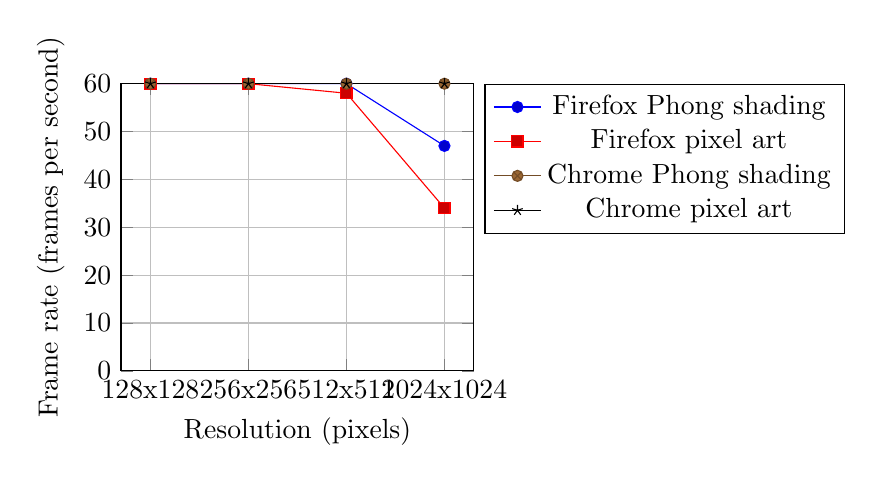
\begin{tikzpicture}
\begin{axis}[
	xlabel={Resolution (pixels)},
	ylabel={Frame rate (frames per second)},
	ymin = 0,
	ymax = 60,
	width = 0.5\textwidth,
	xtick = data,
	ytick = {0,10,...,60},
	grid = major,
	symbolic x coords={128x128, 256x256, 512x512, 1024x1024},
	legend pos = outer north east
]
\addplot coordinates {(128x128, 60) (256x256, 60) (512x512, 60) (1024x1024, 47)};
\addplot coordinates {(128x128, 60) (256x256, 60) (512x512, 58) (1024x1024, 34)};
\addplot coordinates {(128x128, 60) (256x256, 60) (512x512, 60) (1024x1024, 60)};
\addplot coordinates {(128x128, 60) (256x256, 60) (512x512, 60) (1024x1024, 60)};
\legend{Firefox Phong shading,Firefox pixel art,Chrome Phong shading,Chrome pixel art}
\end{axis}
\end{tikzpicture}
\caption{Frame rate while rendering a single reduced-polygon Stanford dragon on a NVIDIA GeForce GTX 765M GPU.}
\label{fig:graph1}
\end{figure}

The maximum frame rate recorded was 60FPS. This is because both browsers I tested with update the WebGL canvas once per screen refresh; as my screen refresh rate is 60Hz, the render code was called 60 times per second.

This limit proved to be detrimental when testing on Chrome, as its WebGL renderer easily maintained 60FPS at all tested resolutions. This made it impossible to evaluate the performance difference between my pixel art shader and the Phong shader. In order to collect useful results, I simulated an increase in scene complexity and resolution by rendering the model 8 times per frame; this gave the results seen in Figure~\ref{fig:graph2}.

\begin{figure}[h!]
\centering
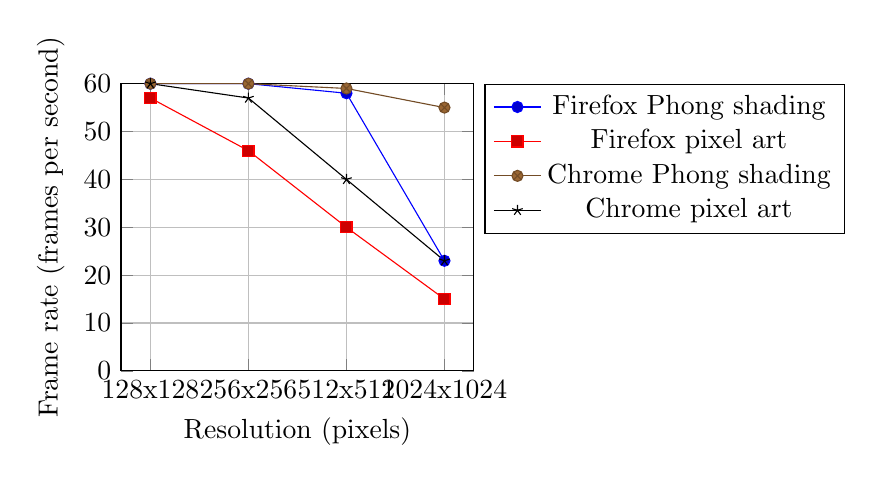
\begin{tikzpicture}
\begin{axis}[
	xlabel={Resolution (pixels)},
	ylabel={Frame rate (frames per second)},
	ymin = 0,
	ymax = 60,
	width = 0.5\textwidth,
	xtick = data,
	ytick = {0,10,...,60},
	grid = major,
	symbolic x coords={128x128, 256x256, 512x512, 1024x1024},
	legend pos = outer north east
]
\addplot coordinates {(128x128, 60) (256x256, 60) (512x512, 58) (1024x1024, 23)};
\addplot coordinates {(128x128, 57) (256x256, 46) (512x512, 30) (1024x1024, 15)};
\addplot coordinates {(128x128, 60) (256x256, 60) (512x512, 59) (1024x1024, 55)};
\addplot coordinates {(128x128, 60) (256x256, 57) (512x512, 40) (1024x1024, 23)};
\legend{Firefox Phong shading,Firefox pixel art,Chrome Phong shading,Chrome pixel art}
\end{axis}
\end{tikzpicture}
\caption{Frame rate while rendering 8 copies of the reduced-polygon Stanford dragon on a NVIDIA GeForce GTX 765M GPU.}
\label{fig:graph2}
\end{figure}

I repeated this on my desktop, with a NVIDIA GeForce GTX 560Ti GPU, and identical browsers. The results are shown in Figure~\ref{fig:graph3}.

\begin{figure}[h!]
\centering
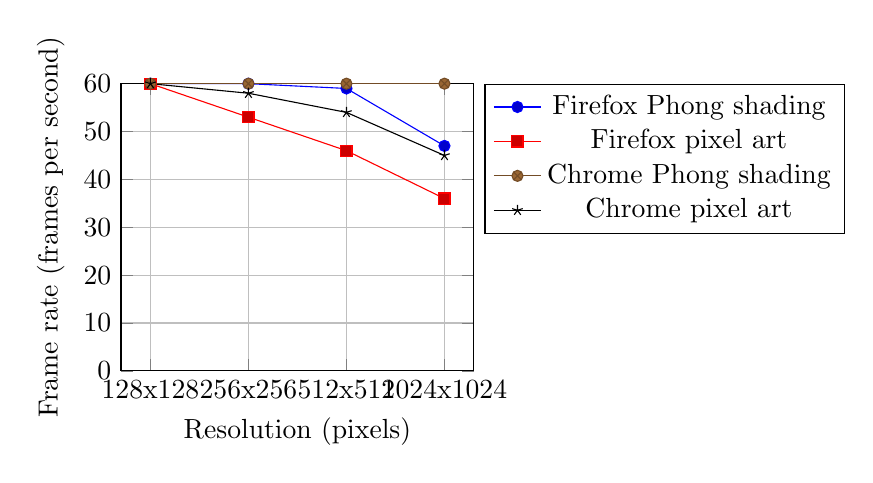
\begin{tikzpicture}
\begin{axis}[
	xlabel={Resolution (pixels)},
	ylabel={Frame rate (frames per second)},
	ymin = 0,
	ymax = 60,
	width = 0.5\textwidth,
	xtick = data,
	ytick = {0,10,...,60},
	grid = major,
	symbolic x coords={128x128, 256x256, 512x512, 1024x1024},
	legend pos = outer north east
]
\addplot coordinates {(128x128, 60) (256x256, 60) (512x512, 59) (1024x1024, 47)};
\addplot coordinates {(128x128, 60) (256x256, 53) (512x512, 46) (1024x1024, 36)};
\addplot coordinates {(128x128, 60) (256x256, 60) (512x512, 60) (1024x1024, 60)};
\addplot coordinates {(128x128, 60) (256x256, 58) (512x512, 54) (1024x1024, 45)};
\legend{Firefox Phong shading,Firefox pixel art,Chrome Phong shading,Chrome pixel art}
\end{axis}
\end{tikzpicture}
\caption{Frame rate while rendering 8 copies of the reduced-polygon Stanford dragon on a NVIDIA GeForce GTX 560Ti GPU.}
\label{fig:graph3}
\end{figure}

The total number of polygons rendered was just under 700,000 per frame. Modern video games often display millions, or even tens of millions, of polygons per scene at resolutions of 1920$\times$1080 and above -- my system would be inadequate for use in such a situation. However, due to the detail loss inherent in palette quantisation and the common practice of scaling pixel art up before rendering it in order for the viewer to more easily appreciate the pixel-level detail, such high polygon counts and resolutions would not be required for many use cases of the system.

As the aesthetic aspect of the project was important, I performed some informal tests to roughly gauge the effectiveness of parts of the project.

I found five people who volunteered to test parts of the system. Two of those were familiar with pixel art already through playing video games.

I asked them to compare two images, one which used a particular technique and one which did not, and say which they thought was clearer, and which they preferred. I randomised the order of the images each time to avoid any bias. An example is shown in Figure~\ref{fig:outlinecomparison}.

\begin{figure}[h!]
\centering
\includegraphics[width=0.5\textwidth]{outlinecomparison}
\caption{Black outlines on the left compared with coloured outlines on the right.}
\label{fig:outlinecomparison}
\end{figure}

Overall, I found that in most cases, three or more participants preferred the appearance of models shaded with pixel art techniques rather than those shaded without them. However, the reverse was true for clarity; in most cases, the additional pixel art features such as dithering made the images less clear. For example, three people found a Phong shaded dragon clearer than the pixel art dragon (using the image in Figure~\ref{fig:shadeddragon}).

I found there was a large difference in opinions between participants who were familiar with pixel art already and those who were not. Those familiar with pixel art preferred the images with additional pixel art features in over 80\% of cases, while those unfamiliar with it were more evenly split.

Without formal human testing, I cannot be certain that my project was successful; I did not treat the above informal study as a measure of success, though the results from it were encouraging.

As I chose to emulate the pixel art style used in \textit{Pok\'{e}mon Black 2/White 2}, I attempted to recreate sprites from those games. The results are shown in Figure~\ref{fig:scolipedecomparison} and Figure~\ref{fig:eeveecomparison}.

\begin{figure}[h!]
\centering
\includegraphics[width=\textwidth]{scolipedecomparison}
\caption{From left to right: Scolipede rendered with an automatically-selected palette, Scolipede rendered with the original pixel art's palette, and Scolipede's original art from \textit{Pok\'{e}mon Black 2/White 2}.}
\label{fig:scolipedecomparison}
\end{figure}

\begin{figure}[h!]
\centering
\includegraphics[width=0.5\textwidth]{eeveecomparison}
\caption{A model of `Eevee' from \textit{Pok\'{e}Park 2} rendered using the pixel art shader, and Eevee's original art from \textit{Pok\'{e}mon Black 2/White 2}.}
\label{fig:eeveecomparison}
\end{figure}

I created histograms for the frequency of each colour normalised for the non-transparent area of each sprite for both the rendered and hand-drawn images, and computed the differences between them. These histograms are shown in Figure~\ref{fig:scolipedehistogram} and Figure~\ref{fig:eeveehistogram}.

\begin{figure}[h!]
\centering
\includegraphics[width=\textwidth]{histogram1}
\caption{Histograms comparing the normalised frequencies of each colour in the rendered image of Scolipede and the hand-drawn art.}
\label{fig:scolipedehistogram}
\end{figure}

\begin{figure}[h!]
\centering
\includegraphics[width=0.728\textwidth]{histogram2}
\caption{Histograms comparing the normalised frequencies of each colour in the rendered image of Eevee and the hand-drawn art.}
\label{fig:eeveehistogram}
\end{figure}

The differences between the histograms reflect the discrepancies between the computer-generated pixel art and the hand-drawn pixel art; the following paragraphs explain these differences.

The models I used have slightly different proportions and pose than the game sprites; for example, Scolipede's horns and tail are thinner in the model, while Eevee's pose is different. Assuming the 3D model has the correct proportions, Scolipede's sprite shows how the pixel art form modifies proportions for clarity; my detail preservation algorithm is not flexible enough to imitate this. Interestingly, note how the silhouette of the horns and tail on the 3D model render is proportionally similar to the area within the outline on the hand-drawn sprite -- rendering the outline on the outside of the model makes the proportions of the horns and tail match the hand-drawn art better, but also makes parts such as the legs look unnaturally bulbous, as in Figure~\ref{fig:bulbous}.

\begin{figure}[h!]
\centering
\includegraphics[width=0.333\textwidth]{bulbous}
\caption{Scolipede rendered with the outline on the outside of the model.}
\label{fig:bulbous}
\end{figure}

Ignoring discrepancies in the model, there are a few further apparent differences between the rendered and hand-drawn versions. The most noticeable is that the rendered sprites have fewer outlines. For example, Eevee's sprite lacks outlining on its mane and between its toes. In addition, both Scolipede's and Eevee's rendered sprites use about 40\% less black in outlines, as can be seen in the histograms in Figure~\ref{fig:scolipedehistogram} and Figure~\ref{fig:eeveehistogram}. This shows that the outlining algorithm is a possible area of improvement; for example, a better algorithm could take into account the texture as well as the depth and normals.

The second is that the rendered sprites use more colours for shading than the hand-drawn sprites; the rendered Scolipede appropriates the blend between red and purple used at the edge of the rings as an additional shade of red, as is evidenced by the spike in the difference histogram in Figure~\ref{fig:scolipedehistogram}. This is because the shading algorithm treats all colours in the palette equally in order to approximate the shading as closely as possible, while a human pixel artist reserves certain colours for certain parts of the subject. The latter approach is useful when `palette swapping', a technique commonly used in video games to create variations of characters, is used (see Figure~\ref{fig:shinyscolipede}); if palette colours are associated with actual colours, palette swaps can be created by modifying the palette without changing the bitmap.

Interestingly, the rendered sprite does not use one of the colours from the hand-drawn sprite, a shade of dark red (seen in Figure~\ref{fig:scolipedehistogram} between the grey and purple bars). This is due to the rigid shading algorithm; none of the Phong shading levels for any colour in the texture were matched to that particular shade of red, which is used as an additional outline colour in the hand-drawn sprite.

\begin{figure}[h!]
\centering
\includegraphics[width=0.667\textwidth]{shinyscolipede}
\caption{`Shiny Scolipede', an example of a palette swap in \textit{Pok\'{e}mon Black 2/White 2}. Note how the shading on the left, rendered, sprite is different to that in Figure~\ref{fig:scolipedecomparison} while the shading on the right, hand-drawn, sprite is identical.}
\label{fig:shinyscolipede}
\end{figure}

Finally, the lighting is different between the rendered and hand-drawn sprites. This is down to two reasons -- I did not implement shadowing, so parts of the model that should be in shadow, such as Eevee's tail and back leg, are lit. This is made obvious in Figure~\ref{fig:eeveehistogram}; the colours that are used more commonly in the render than in the hand-drawn art are the lit colours and the lighter outline colours, while the shadowed colours are neglected in the render. Additionally, a human artist can use `artistic license' when shading, while my system shades rigidly based only on light source position. For example, Scolipede's foreground horn on the hand-drawn sprite is completely illuminated, implying the light source is to the side, in the direction of the viewer; most of the other shading implies the light source should be above it. Although incorrect, illuminating the foreground horn and shading the background horn gives a sense of depth. My shading algorithm does not reproduce this technique.

As with any computer-generated emulation of a hand-drawn art style, the output of the program is not entirely correct. However, in the intended use-case of real-time pixel art rendering, the smooth animation produced hides many of the imperfections. By the art form's nature, errors are generally only a few pixels in size; displaying these in a real-time animation means each error is only visible for a fraction of a second. These two factors mean that most errors are difficult for viewers to discern.

While I was implementing the project, I kept a suite of unit tests up-to-date for both my JavaScript and GLSL functions. This allowed me to ensure critical parts of the system, such as the code to pack floating-point numbers into colours, would work correctly. I made sure to cover edge cases such as 1/256 as well as ordinary use cases.

\chapter{Conclusion}

The implementation of the project was generally successful. The system's output is a good approximation of hand-drawn pixel art; the project, or at least some of the methods used in the implementation, has the potential to see use by video game developers wishing to add a pixel art look to a game. As mentioned in the introduction, using 3D models rendered as pixel art has several advantages over hand-drawing the art in both visuals and production effort.

The main failure of the project was due to not strictly keeping up with my schedule. Falling behind led to a lack of time for evaluation, which in turn meant I cannot claim to have met my success criteria; in hindsight, I would have cut part of the implementation short in order to have more time for evaluation, potentially returning to complete it afterwards.

Potential extensions to the project that could be performed in the future include porting the code to a library or engine more commonly used in game development; WebGL is very suitable for demonstrating the project and for portability, but is rarely used for video games.

The shading system could also be improved; two things mentioned in Chapter~4 are shadowing and associating particular colours with parts of the model. Shadowing can be implemented using an algorithm such as shadow mapping~\cite{Williams:1978:CCS:965139.807402}, while colour association could be performed by dividing palette colours into sets, mapping certain texture regions to palette subsets.

\bibliography{references}
\bibliographystyle{plain}

\cleardoublepage

\appendix

\chapter{OpenGL ES Example}

\label{app:gles}

\begin{lstlisting}[caption =Building a texture containing the model outline]
function renderOutline(model) {
	// render to a framebuffer rather than to the screen
	gl.bindFramebuffer(gl.FRAMEBUFFER, screenFramebuffer);
	
	// render normals to a texture
	gl.framebufferTexture2D(gl.FRAMEBUFFER, gl.COLOR_ATTACHMENT0, gl.TEXTURE_2D, normalTexture, 0);
	gl.clear(gl.COLOR_BUFFER_BIT | gl.DEPTH_BUFFER_BIT);
	drawModel(normalShader, model);
	
	// render depth to a texture
	gl.framebufferTexture2D(gl.FRAMEBUFFER, gl.COLOR_ATTACHMENT0, gl.TEXTURE_2D, depthTexture, 0);
	gl.clear(gl.COLOR_BUFFER_BIT | gl.DEPTH_BUFFER_BIT);
	gl.useProgram(depthShader);
	drawModel(depthShader, model);
	
	// set up outline shader uniforms
	gl.useProgram(outlineShader);
	gl.activeTexture(gl.TEXTURE0);
	gl.bindTexture(gl.TEXTURE_2D, depthTexture);
	gl.uniform1i(outlineShader.depthTexture, 0);
	gl.activeTexture(gl.TEXTURE1);
	gl.bindTexture(gl.TEXTURE_2D, normalTexture);
	gl.uniform1i(outlineShader.normalTexture, 1);
	gl.uniform2i(outlineShader.textureSize, screenBufferWidth(), screenBufferHeight());
	
	//render outlines to a texture
	gl.framebufferTexture2D(gl.FRAMEBUFFER, gl.COLOR_ATTACHMENT0, gl.TEXTURE_2D, edgeTexture, 0);
	gl.clear(gl.COLOR_BUFFER_BIT | gl.DEPTH_BUFFER_BIT);
	drawRectangle(outlineShader);
	
	// unbind framebuffer and render to the screen again
	gl.framebufferTexture2D(gl.FRAMEBUFFER, gl.COLOR_ATTACHMENT0, gl.TEXTURE_2D, screenTexture, 0);
	gl.bindFramebuffer(gl.FRAMEBUFFER, null);
}
\end{lstlisting}

\chapter{CIEDE2000 Colour Difference}

\label{app:ciede2000}

The CIEDE2000 difference $\Delta E_{00}^*$ between two colours in the CIELAB colour space $(L^*_1, a^*_1, b^*_1)$ and $(L^*_2, a^*_2, b^*_2)$ is given by the following equation:

\begin{equation}
\Delta E_{00} = \sqrt{ \left(\frac{\Delta L'}{k_L S_L}\right)^2 + \left(\frac{\Delta C'}{k_C S_C}\right)^2 + \left(\frac{\Delta H'}{k_H S_H}\right)^2 + R_T \frac{\Delta C'}{k_C S_C}\frac{\Delta H'}{k_H S_H} }
\end{equation}
The terms used in the equation are given by the following equations (all angles are in degrees):
\begin{align}
\Delta L^\prime &= L^*_2 - L^*_1 \\
\bar{L}&= \frac{L^*_1 + L^*_2}{2} \quad \bar{C} = \frac{C^*_1 + C^*_2}{2} \\
a_1^\prime &= a_1^* + \frac{a_1^*}{2} \left( 1 - \sqrt{\frac{\bar{C}^7}{\bar{C}^7 + 25^7}} \right) \\
a_2^\prime &= a_2^* + \frac{a_2^*}{2} \left( 1 - \sqrt{\frac{\bar{C}^7}{\bar{C}^7 + 25^7}} \right) \\
C_1^\prime &= \sqrt{a_1^{'^2} + b_1^{*^2}} \\
C_2^\prime &= \sqrt{a_2^{'^2} + b_2^{*^2}} \\
\bar{C}^\prime &= \frac{C_1^\prime + C_2^\prime}{2} \\
\Delta{C'}&=C'_2-C'_1 \\
h_1^\prime&=\text{atan2} (b_1^*, a_1^\prime) \mod 360^\circ \\
h_2^\prime&=\text{atan2} (b_2^*, a_2^\prime) \mod 360^\circ \\
\Delta h' &= \begin{cases}
h_2^\prime - h_1^\prime & \left| h_1^\prime - h_2^\prime \right| \leq 180^\circ \\
h_2^\prime - h_1^\prime + 360^\circ & \left| h_1^\prime - h_2^\prime \right| > 180^\circ, h_2^\prime \leq h_1^\prime \\
h_2^\prime - h_1^\prime - 360^\circ & \left| h_1^\prime - h_2^\prime \right| > 180^\circ, h_2^\prime > h_1^\prime
\end{cases} \\
\Delta H^\prime &= 2 \sqrt{C_1^\prime C_2^\prime} \sin (\Delta h^\prime/2) \\
\bar{H}^\prime&=\begin{cases}
(h_1^\prime + h_2^\prime + 360^\circ)/2 & \left| h_1^\prime - h_2^\prime \right| > 180^\circ \\
(h_1^\prime + h_2^\prime)/2 & \left| h_1^\prime - h_2^\prime \right| \leq 180^\circ
\end{cases} \\
T &= 1 - 0.17 \cos ( \bar{H}^\prime - 30^\circ )\nonumber\\
&\qquad+ 0.24 \cos (2\bar{H}^\prime)\nonumber\\
&\qquad+ 0.32 \cos (3\bar{H}^\prime + 6^\circ )\nonumber\\
&\qquad- 0.20 \cos (4\bar{H}^\prime - 63^\circ) \\
S_L &= 1 + \frac{0.015 \left( \bar{L} - 50 \right)^2}{\sqrt{20 + {\left(\bar{L} - 50 \right)}^2} } \\
S_C &= 1+0.045 \bar{C}^\prime \\
S_H &= 1+0.015 \bar{C}^\prime T \\
R_T &= -2 \sqrt{\frac{\bar{C}'^7}{\bar{C}'^7+25^7}} \sin \left[ 60^\circ \cdot \exp \left( -\left[ \frac{\bar{H}'-275^\circ}{25^\circ} \right]^2 \right) \right]
\end{align}

\chapter{Constructing the CIEDE2000 Cache}
\label{app:cache}
\begin{lstlisting}
#define PI 3.141592653589793238462643383279
precision highp float;
uniform sampler2D palette;
uniform mat3 rgbConversion;
uniform int paletteSize;
// the precision of the cache
const int bits = 8;

float linearise(float c) {
	if (c <= 0.04045) {
		return (c / 12.92);
	} else {
		return pow((c + 0.055) / 1.055, 2.4);
	}
}

float labf(float c) {
	if (c > 0.008856) {
		return pow(c, 1.0/3.0);
	} else {
		return 7.787 * c + 0.1379;
	}
}

float dsin(float degrees) {
	return sin(degrees / 180.0 * PI);
}

float dcos(float degrees) {
	return cos(degrees / 180.0 * PI);
}

float datan(float y, float x) {
	return atan(y, x) / PI * 180.0;
}

float ciede2000(vec3 lab1, vec3 lab2) {
	float cavg = (length(lab1.yz) + length(lab2.yz)) / 2.0;
	float cavg7 = cavg * cavg * cavg * cavg * cavg * cavg * cavg;
	float g = 0.5 * (1.0 - sqrt(cavg7 / (cavg7 + 6103515625.0)));
	float ap1 = (1.0 + g) * lab1.y;
	float ap2 = (1.0 + g) * lab2.y;
	float cp1 = sqrt(ap1 * ap1 + lab1.z * lab1.z);
	float cp2 = sqrt(ap2 * ap2 + lab2.z * lab2.z);
	float h1 = 0.0;
	if (lab1.z != 0.0 || ap1 != 0.0) {
		h1 = datan(lab1.z, ap1);
		if (h1 < 0.0) {
			h1 += 360.0;
		}
	}
	float h2 = 0.0;
	if (lab2.z != 0.0 || ap2 != 0.0) {
		h2 = datan(lab2.z, ap2);
		if (h2 < 0.0) {
			h2 += 360.0;
		}
	}
	float dl = lab2.x - lab1.x;
	float dc = cp2 - cp1;
	float dh = 0.0;
	if (cp1 != 0.0 && cp2 != 0.0) {
		dh = h2 - h1;
		if (dh < -180.0) {
			dh += 360.0;
		} else if (dh > 180.0) {
			dh -= 360.0;
		}
	}
	float dch = 2.0 * sqrt(cp1 * cp2) * dsin(dh / 2.0);
	float lavg = (lab1.x + lab2.x) / 2.0;
	float cpavg = (cp1 + cp2) / 2.0;
	float havg = h1 + h2;
	if (cp1 != 0.0 && cp2 != 0.0) {
		if (abs(h1 - h2) < 180.0) {
			havg = (h1 + h2) / 2.0;
		} else {
			if (h1 + h2 < 360.0) {
				havg = (h1 + h2 + 360.0) / 2.0;
			} else {
				havg = (h1 + h2 - 360.0) / 2.0;
			}
		}
	}
	float t = 1.0 - 0.17 * dcos(havg - 30.0) + 0.24 * dcos(2.0 * havg) + 0.32 * dcos(3.0 * havg + 6.0) - 0.2 * dcos(4.0 * havg - 63.0);
	float sqterm = ((havg - 275.0) / 25.0);
	float dtheta = 30.0 * exp(-(sqterm * sqterm));
	float cpavg7 = cpavg * cpavg * cpavg * cpavg * cpavg * cpavg * cpavg;
	float rc = 2.0 * sqrt(cpavg7 / (cpavg7 + 6103515625.0));
	float lavgp = (lavg - 50.0) * (lavg - 50.0);
	float sl = 1.0 + (0.015 * lavgp) / sqrt(20.0 + lavgp);
	float sc = 1.0 + 0.045 * cpavg;
	float sh = 1.0 + 0.015 * cpavg * t;
	float rt = -dsin(2.0 * dtheta) * rc;
	float de = sqrt((dl / sl) * (dl / sl) + (dc / sc) * (dc / sc) + (dch / sh) * (dch / sh) + rt * (dc / sc) * (dch / sh));
	return de;
}

vec3 srgbToCiexyz(vec3 srgb) {
	vec3 linearRgb = vec3(linearise(srgb.r), linearise(srgb.g), linearise(srgb.b));
	return linearRgb * rgbConversion;
}

vec3 srgbToCielab(vec3 srgb) {
	vec3 ciexyz = srgbToCiexyz(srgb);
	// adjust for sRGB white point before calling labf
	float fX = labf(ciexyz.x / 0.95047);
	float fY = labf(ciexyz.y);
	float fZ = labf(ciexyz.z / 1.08883);
	vec3 cielab = vec3(max(116.0 * fY - 16.0, 0.0), 500.0 * (fX - fY), 200.0 * (fY - fZ));
	return cielab;
}

vec4 getClosestColour(vec4 colour) {
	float bestDist = -1.0;
	vec4 bestColour;
	vec4 paletteColour;
	// GLSL does not support comparing loop count to a variable, so just loop to a safe number and break when necessary
	for (int i = 0; i < 64; i++) {
		paletteColour = texture2D(palette, vec2(float(i) / float(paletteSize), 0));
		float dist = ciede2000(srgbToCielab(colour.rgb), srgbToCielab(paletteColour.rgb));
		if (dist < bestDist || bestDist < 0.0) {
			bestColour = paletteColour;
			bestDist = dist;
		}
		if (i >= paletteSize) {
			break;
		}
	}
	return bestColour;
}

void main(void) {
	float size = pow(2.0, float(bits));
	float sqrtSize = sqrt(size);
	// since we're building a cache texture, the colour to quantise is a function of the fragment coordinates
	float r = mod(gl_FragCoord.x, size) / (size - 1.0);
	float g = mod(gl_FragCoord.y, size) / (size - 1.0);
	float b = (floor(gl_FragCoord.x / size) / (sqrtSize - 1.0) + floor(gl_FragCoord.y / size)) / (sqrtSize - 1.0);
	gl_FragColor = getClosestColour(vec4(r, g, b, 1.0));
}
\end{lstlisting}

\chapter{Outline Colour Quantisation}
\label{app:outlines}
\begin{lstlisting}
vec4 getEdgeColour(vec4 colour) {
	vec2 coord = gl_FragCoord.xy / vec2(textureSize);
	vec2 lcoord = coord - vec2(1.0 / float(textureSize.x), 0.0);
	vec2 rcoord = coord + vec2(1.0 / float(textureSize.x), 0.0);
	vec2 dcoord = coord - vec2(0.0, 1.0 / float(textureSize.y));
	vec2 ucoord = coord + vec2(0.0, 1.0 / float(textureSize.y));
	float ll = 100.0;
	if (texture2D(edgeTexture, lcoord).r < edgeThreshold && unpack(texture2D(depthTexture, lcoord)) < 1.0) {
		ll = srgbToCielab(getMatchingColour(getPhongColour(lcoord)).rgb).x;
	}
	float rl = 100.0;
	if (texture2D(edgeTexture, rcoord).r < edgeThreshold && unpack(texture2D(depthTexture, rcoord)) < 1.0) {
		rl = srgbToCielab(getMatchingColour(getPhongColour(rcoord)).rgb).x;
	}
	float dl = 100.0;
	if (texture2D(edgeTexture, dcoord).r < edgeThreshold && unpack(texture2D(depthTexture, dcoord)) < 1.0) {
		dl = srgbToCielab(getMatchingColour(getPhongColour(dcoord)).rgb).x;
	}
	float ul = 100.0;
	if (texture2D(edgeTexture, ucoord).r < edgeThreshold && unpack(texture2D(depthTexture, ucoord)) < 1.0) {
		ul = srgbToCielab(getMatchingColour(getPhongColour(lcoord)).rgb).x;
	}
	vec4 paletteColour = getMatchingColour(colour);
	float l = srgbToCielab(paletteColour.rgb).x + minEdgeLDifference;
	if (l >= ll || l >= rl || l >= dl || l >= ul) {
		for (int i = 0; i < 20; i++) {
			colour = colour * vec4(0.9, 0.9, 0.9, 1.0);
			paletteColour = getMatchingColour(colour);
			l = srgbToCielab(paletteColour.rgb).x + minEdgeLDifference;
			if (l < ll && l < rl && l < dl && l < ul) {
				break;
			}
		}
	}
	return paletteColour;
}
\end{lstlisting}

\end{document}
